\documentclass{article}
\usepackage[preprint]{neurips_2025}
\usepackage[T1]{fontenc}
\usepackage[utf8]{inputenc}
\usepackage{graphicx}
\usepackage{booktabs}
\usepackage{url}
\usepackage{hyperref}
\title{Aisha Agent: A Source-Grounded Municipal Information Harness\\Compulsory 2: Plan and Walking Skeleton}
\author{KIUA-2003 project group\\University of Inland Norway}
\begin{document}
\maketitle
\begin{abstract}
Aisha Agent addresses recurring searches for municipal service information in Hamar, Innlandet. Its walking skeleton combines approved local excerpts, constrained model selection, evidence verification, and cited output. It is deliberately extractive: it neither crawls municipal websites during a query nor guarantees factual completeness. This report specifies the problem, implemented architecture, reproducible path, preliminary verification, and remaining delivery dependencies. The current evidence supports an operating skeleton, but not a claim of submission readiness: the supplied template, compiled page count, confirmed meeting evidence, and dated demonstration schedule remain unverified.
\end{abstract}

\section{Problem Description and Local Relevance}
Residents repeatedly need information about building applications, water, parking, and other municipal services. Finding the appropriate official page and identifying a relevant passage creates recurring information work. Aisha Agent provides a local interface for service search and a source-linked answer, aligned with the assignment's emphasis on Innlandet and information accessibility \cite{assignment}. The system is a student prototype, not an official municipal service. Its output is one selected, reviewed paragraph with an official source reference, or a clarification/refusal when evidence is inadequate. This narrower output makes support checkable while limiting unsupported generation. The project does not establish that the selected services represent all resident needs; no user interview or survey result is asserted.

\section{Target Users and Recurring Information Need}
Intended users are residents and others seeking general, non-personal information about Hamar services. A representative question is ``Hva kan jeg bygge uten å søke?'' Users should be able to locate an official building-application source without supplying names, addresses, case numbers, or personal circumstances. Repeated access to general information is the target workflow; individual case advice, legal interpretation, and processing applications are outside scope. The interface separates ordinary search from the AI path and retains visible official links. Desktop, tablet, and mobile layouts support different access contexts. These are design intentions supported by browser checks, not empirical claims about usability, accessibility for every user, or social benefit.

\section{Success Criteria and Verifiable Outputs}
Success for the skeleton means that approved or explicitly synthetic input passes through multiple automatic stages and produces machine-checkable output. A positive real-source result must retain source identity, paragraph identity, provenance, and an exact match between its claim, evidence quotation, and a complete approved paragraph. Unsupported or ineligible input must not be published as a grounded answer. A correction is permitted once, followed by independent re-verification; unresolved findings block publication.

Four mandatory technical minima are evidenced in code \cite{repository}. (1) JSON output and citations can be checked against input paragraphs, using the CLI and evidence verifier. (2) Source eligibility, retrieval/context selection, model selection, and verification are separate stages rather than one prompt. (3) The harness uses local files, a search index, JSON storage, and the loopback Ollama HTTP tool. (4) Once invoked, execution proceeds automatically through these stages, including the bounded correction decision. Human source approval occurs before this automatic path; it is not represented as an autonomous source-admission decision. Test success measures these criteria, not universal truth or complete municipal coverage.

\section{Agentic Harness Architecture}
The application uses Python and a local Ollama provider. Python 3.12.10 is the recorded evaluation interpreter. The reviewed catalog contains eight documents and 39 approved paragraphs; its approvals were reviewed on 2026-10-21 and expire on 2026-10-28 \cite{evidence}. Eligibility is checked before use. Raw HTML acquisition and import are currently disabled. Search retrieves from the local approved collection, not from a live municipal website. Figure~\ref{fig:workflow} summarizes the implemented path. The architecture is a deterministic orchestrator with a constrained model stage, not a collection of independently acting conversational agents.
\begin{figure}[ht]
\centering
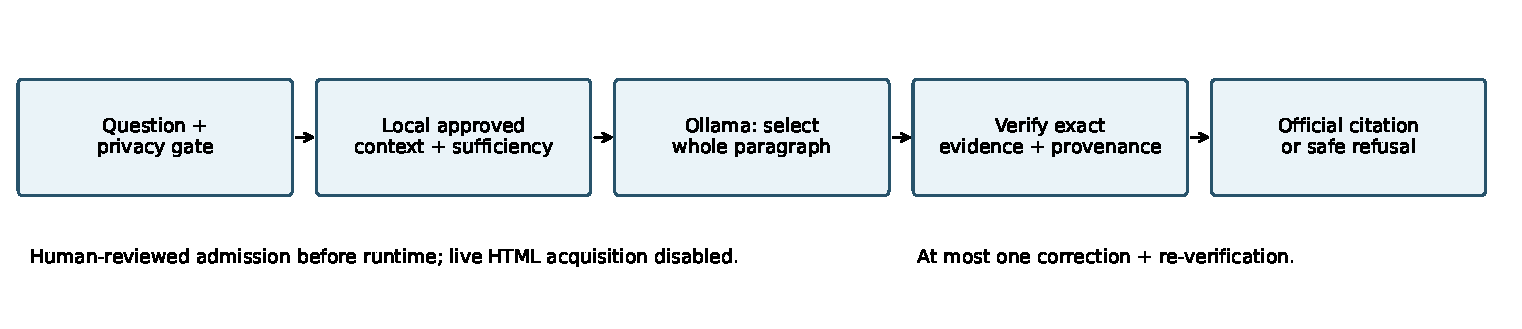
\includegraphics[width=\linewidth]{../figures/aisha-workflow.pdf}
\caption{Aisha Agent workflow. Human source admission precedes runtime; automatic selection and verification yield a citation or safe refusal. One correction is followed by mandatory re-verification.}
\label{fig:workflow}
\end{figure}
The browser calls the local Python service; Ollama is contacted on loopback. The application's web interface remains local and no public deployment or tunnel is part of this skeleton. Source restrictions, dates, and privacy controls are retained by this report task.

\section{Context Engineering, Tools and Autonomous Stages}
The context is a bounded set of approved source paragraphs selected by the local search and sufficiency rules. External source text is untrusted data, not instructions. In real municipal mode the model selects a complete paragraph through structured output; it does not receive an unrestricted mandate to generate advice or retrieve more sources. The adapter constrains output format, while a separate verifier checks evidence and exact paragraph support. A model response alone is therefore insufficient for publication.

The measured model is \texttt{llama3.2:3b}; configuration uses temperature 0, seed 0, context 4096, and a requested maximum of 700 generated tokens per call. At most two calls are allowed through the correction path. These are per-request limits, not an enforced aggregate token or financial budget. A 90-second timeout can be selected for real runs; it is not a global computation deadline. The model never silently falls back to synthetic data in real-source mode. User-facing errors and insufficient-evidence responses must remain distinguishable from successful grounded output. The local tools and bounded orchestration implement autonomy without permitting arbitrary shell commands or municipal crawling by the model.

\section{Walking Skeleton and Reproducibility}
The repository README contains the setup and context boundaries. From its root, a dependency-free synthetic path is:
\begin{quote}\small\ttfamily
python -X utf8 -m hamar\_agent --fixture fixtures/water-synthetic.json
\end{quote}
This explicit mock-provider path checks orchestration and supported output without claiming to test a real model. A separately recorded execution and command metadata are included under \texttt{comp2/evidence/}. A real-model path, requiring an existing valid approved catalog and the installed model, is:
\begin{quote}\small\ttfamily
python -X utf8 -m hamar\_agent --real-sources --source hamar-byggesak --model llama3.2:3b --ollama-timeout 90
\end{quote}
The CLI source path verifies the service-source workflow; the browser harness separately verifies question-based retrieval and the official building citation. The ignored municipal catalog is not distributed by a Git clone. Consequently, a new machine can reproduce the synthetic path immediately, while reproducing municipal mode additionally requires authorized access to eligible local excerpts. After expiration the real path should refuse; extending dates simply to reproduce a result is not allowed. Detailed setup, expected checks, and commands appear in the package README. No new source retrieval is needed or authorized.

\section{Preliminary Verification Results}
Table~\ref{tab:results} selects results recorded on 2026-10-23, retaining their original denominators \cite{evidence,results}. These are different test families and must not be pooled into an overall accuracy percentage. The real-model suite includes expected refusals and a repeat. The independent archived-output audit checks 17 saved positive outputs from the earlier historical suite; it is not a rerun of the later model batch. The summary's partial \texttt{grounded\_claims} field is not used as the count of saved outputs. Browser evidence confirms three viewports and visible official links, without establishing human-rated accessibility.
\begin{table}[ht]
\centering\small
\begin{tabular}{lr}
\toprule
Measure & Observed / evaluated \\
\midrule
Offline regression & 282/282 \\
Real Ollama cases & 23/23 \\
Saved positive outputs & 17/17 \\
Responsive Chrome layouts & 3/3 \\
Insufficient-evidence refusals & 4/4 \\
Permission and prompt boundaries & 10/10 \\
Approval and endpoint gates & 15/15 \\
\bottomrule
\end{tabular}

\caption{Selected preliminary verification, 2026-10-23. Exact-source support is not semantic factual accuracy. Source files and limitations are supplied in the bilingual CSV/Markdown tables.}
\label{tab:results}
\end{table}
A separate performance experiment completed only 14 of 20 planned calls before its thermal safety stop: 12 sequential calls and two concurrent calls. Sequential median latency was 1511.1545 ms and nearest-rank p95 was 2103.674 ms. The small concurrent sample is not a throughput estimate. Reported token totals for this instrumented series were 4120 input and 1716 generated tokens. Energy and monetary cost were not measured. The supporting response-time figure is retained outside the main report to avoid obscuring the skeleton's acceptance criteria. No human feedback is fabricated, and detailed stress testing is reserved for the final white paper.

\section{Project Timeline and Milestones}
The demonstration and submission dates are not supplied in the available authoritative text. The following is a proposed backward schedule, not a confirmed calendar or evidence of meetings. Let $D$ be the demonstration date, to be confirmed by the students: $D-21$ days, confirm requirements, privacy boundary, and source availability; $D-14$, reproduce the skeleton and review provenance; $D-7$, complete relevant regressions and resolve report/meeting evidence; $D-3$, compile the supplied template and verify the main-text and prompt limits; $D-1$, rehearse an explicit synthetic demonstration and check valid real-mode availability; $D$, demonstrate input, stages, citation, and refusal. The actual submission deadline must be inserted and the plan reconciled with it before delivery. Existing implementation and evaluation records show progress, but cannot substitute for this missing planning confirmation.

\section{Risks and Mitigation}
The most immediate risks are stale approvals, missing local catalog/model, irrelevant but textually supported selections, and overinterpretation of verification. Mitigations are eligibility checks, fail-closed startup and execution, bounded selection, independent verification, and explicit disclosure of incomplete coverage. Full-paragraph matching demonstrates traceability rather than independent truth or semantic entailment. Model failures do not justify publishing unverified output.

The assignment prohibits processing identifying personal data even when publicly available. Historical transient HTML handling therefore remains a compliance concern; present acquisition is disabled rather than silently treating user source approval as a waiver. Current eligible excerpts are limited to reviewed non-personal service information. Source renewal needs a compliant input process and human review. The current system also lacks a global computation kill switch and aggregate cost budget, and a self-asserted administration role is not authenticated identity. These limitations constrain use and motivate later repairs; they are not disguised as successful safety tests. Local-only operation, session/origin checks, privacy rejection, and publication blocking reduce exposure but do not establish comprehensive security. Controlled stress and causal repair evidence belong primarily to the final report.

\section{Repository and References}
Repository: \url{https://github.com/powerNeron/innlandet-agentic-workflows}. Evidence selection is anchored to commit \texttt{be3884c3bcd5e55f8b5fe5ef9f03505eb7bd94c8}; source results retain their own historical provenance. The package contains bilingual tables generated from one selected dataset, original-byte evidence copies, command records, and an audit/checklist. Students remain responsible for reviewing AI-assisted material. Mandatory meeting provenance, the supplied NeurIPS style, actual compiled lengths, and the dated schedule are explicitly unresolved. This draft is therefore not yet a submission-ready artifact.
\label{maintextend}
\clearpage
\bibliographystyle{plain}
\bibliography{references}
\clearpage
\appendix
\section{Representative Coding-Agent Prompt Excerpts}
\label{promptstart}
These genuine sanitized user instructions are quoted from the evaluation interaction and preserved in \texttt{resultat/english/17\_prompt\_excerpts.md}. They document evidence work, not a complete development transcript.
\begin{quote}
``Do not invent measurements or claim a test was performed when it was not.''

``Do not equate a 100\% test pass rate with 100\% factual accuracy or complete real-world reliability.''

``Do not modify application functionality without separate approval.''

``Do not fabricate missing results or survey responses.''
\end{quote}
Purpose: constrain independent evaluation to reproducible, non-fabricated evidence. Documented outcome: a bilingual evidence package with explicit unresolved safety and submission gaps. Earlier implementation interactions are sanitized summaries in \texttt{docs/prompt-log.md}, not verbatim dialogue; their constraints include synthetic inputs, no network calls, and one revision for the summarizer/verifier interface. No hidden reasoning or reconstructed conversation is supplied. The compiled appendix must be checked against the maximum of two pages.
\label{promptend}
\clearpage
\section{Meeting Evidence Status}
The repository contains eight candidate decision/implementation notes under \texttt{docs/meetings/}, but this audit cannot verify any as a participant-confirmed team meeting. This is not evidence that no meetings occurred. No dates, participants, discussions, or attendance have been invented. \texttt{comp2/appendices/meeting\_reports.md} lists the candidate paths and required confirmation. Genuine meeting reports documenting iterative reasoning remain required before submission; implementation notes alone are not represented as satisfying that requirement.
\end{document}
